\documentclass[a4paper,12pt]{article} % добавить leqno в [] для нумерации слева
\usepackage[a4paper,top=1.3cm,bottom=2cm,left=1.5cm,right=1.5cm,marginparwidth=0.75cm]{geometry}
%%% Работа с русским языком
\usepackage{cmap}					% поиск в PDF
\usepackage{mathtext} 				% русские буквы в фомулах
\usepackage[T2A]{fontenc}			% кодировка
\usepackage[utf8]{inputenc}			% кодировка исходного текста
\usepackage[english,russian]{babel}	% локализация и переносы
\usepackage{multirow}

\usepackage{graphicx}

\usepackage{wrapfig}
\usepackage{tabularx}

\usepackage{hyperref}
\usepackage[rgb]{xcolor}
\hypersetup{
colorlinks=true,urlcolor=blue
}

%%% Дополнительная работа с математикой
\usepackage{amsmath,amsfonts,amssymb,amsthm,mathtools} % AMS
\usepackage{icomma} % "Умная" запятая: $0,2$ --- число, $0, 2$ --- перечисление

%% Номера формул
\mathtoolsset{showonlyrefs=true} % Показывать номера только у тех формул, на которые есть \eqref{} в тексте.

%% Шрифты
\usepackage{euscript}	 % Шрифт Евклид
\usepackage{mathrsfs} % Красивый матшрифт

%% Свои команды
\DeclareMathOperator{\sgn}{\mathop{sgn}}

%% Перенос знаков в формулах (по Львовскому)
\newcommand*{\hm}[1]{#1\nobreak\discretionary{}
{\hbox{$\mathsurround=0pt #1$}}{}}

%% Графики
\usepackage{tikz}
\usepackage{pgfplots}
\pgfplotsset{compat=1.9}

\date{\today}

\begin{document}

\begin{titlepage}
	\begin{center}
		{\large МОСКОВСКИЙ ФИЗИКО-ТЕХНИЧЕСКИЙ ИНСТИТУТ (НАЦИОНАЛЬНЫЙ ИССЛЕДОВАТЕЛЬСКИЙ УНИВЕРСИТЕТ)}
	\end{center}
	\begin{center}
		{\large Физтех-школа аэрокосмических технологий}
	\end{center}
	
	
	\vspace{4.5cm}
	{\huge
		\begin{center}
			{\bf Отчёт о выполнении лабораторной работы 2.5.1}\\
			Измерение коэффициента поверхностного натяжения жидкости
		\end{center}
	}
	\vspace{1cm}
	\begin{center}
		{\large Соболевский Федор Александрович \\
			\vspace{0.2cm}
			Б03-109}
	\end{center}
	\vspace{8cm}
	\begin{center}
		Март 2022
	\end{center}
\end{titlepage}

\section{Аннотация}

В данной работе изучено явление поверхностного натяжения жидкости. Измерена температурная зависимость коэффициента поверхностного натяжения дистиллированной воды с использованием известного коэффициента поверхностного натяжения спирта. С помощью полученных значений определена полная поверхностная энергия и теплота, необходимая для изотермического образования единицы поверхности жидкости при различной температуре.

\section{Теоретические сведения}

\subsection{Явление поверхностного натяжения}

Молекулы жидкости притягиваются друг к другу силами электростатического происхождения, возникающими из-за их взаимной поляризации. Те молекулы, которые находятся в поверхностном слое на границе с газом, притягиваются
в сторону жидкости гораздо сильнее, чем в направлении газа из-за большой разницы плотностей. Вследствие этого молекулы поверхностного слоя обладают большей потенциальной энергией по сравнению с молекулами внутри жидкости. Работа, необходимая для обратимого изотермического образования единицы площади поверхности жидкости, называется коэффициентом поверхностного натяжения и обозначается $\sigma$.

Для исследования термодинамики поверхностного натяжения запишем первое начало термодинамики с учётом $\delta A = -\sigma dF$, где $F$ - площадь поверхности:

\begin{equation}
    \delta Q = dU_F - \sigma dF,
    \label{firstLaw}
\end{equation}

где $U_F$ - полная поверхностная энергия. Перепишем \eqref{firstLaw} с учётом $\delta Q = TdS$:

\begin{equation}
    dU_F = TdS + \sigma dF.
    \label{uf}
\end{equation}

Выразим из \eqref{uf} дифференциал свободной энергии поверхности $d\Psi_F$, зная, что $\Psi_F = U_F - TS$:

\begin{equation}
    d\Psi_F = \sigma dF - SdT.
    \label{dphi}
\end{equation}

Из \eqref{dphi} следует

\begin{equation}
    S = (\frac{\partial\Psi_F}{\partial T})_F
    \label{enthropy}
\end{equation}

и

\begin{equation}
    \sigma = (\frac{\partial\Psi_F}{\partial F})_T.
    \label{sigma}
\end{equation}

Интегрируя \eqref{sigma} с учётом $\Phi_F = 0$ при $F = 0$, получим

\begin{equation}
    \Psi_F = \sigma F.
    \label{phif}
\end{equation}

Подставляя \eqref{phif} в \eqref{enthropy} и используя это соотношение в \eqref{uf}, получим окончательное выражение для полной энергии поверхности:

\begin{equation}
    U_F = (\sigma - T\frac{d\sigma}{dT})F.
\end{equation}

Это выражение можно переписать в виде

\begin{equation}
    \frac{U_F}{F} = \sigma - T\frac{d\sigma}{dT},
    \label{surfaceEnergy}
\end{equation}

где $U_F/F$ - энергия единицы поверхности. 

Введём величину $q$, обозначающую количество теплоты, необходимое для изменения площади поверхности на единицу площади в изотермическом процессе. Из \eqref{firstLaw} с учётом $dU_F = 0$ получим

\begin{equation}
    q = -T\frac{d\sigma}{dT}.
    \label{qu}
\end{equation}

Наличие поверхностного слоя жидкости приводит к различию давлений внутри жидкости и снаружи. Эту разницу давлений можно найти по формуле Лапласа:

\begin{equation}
    \Delta P = \sigma K,
    \label{Laplass}
\end{equation}

где $K$ - кривизна поверхности. Для сферического пузырька радиуса $r$ кривизна поверхности поверхности определяется как $K = 2\sigma/r$.

\subsection{Экспериментальная установка}

\begin{figure}
    \centering
    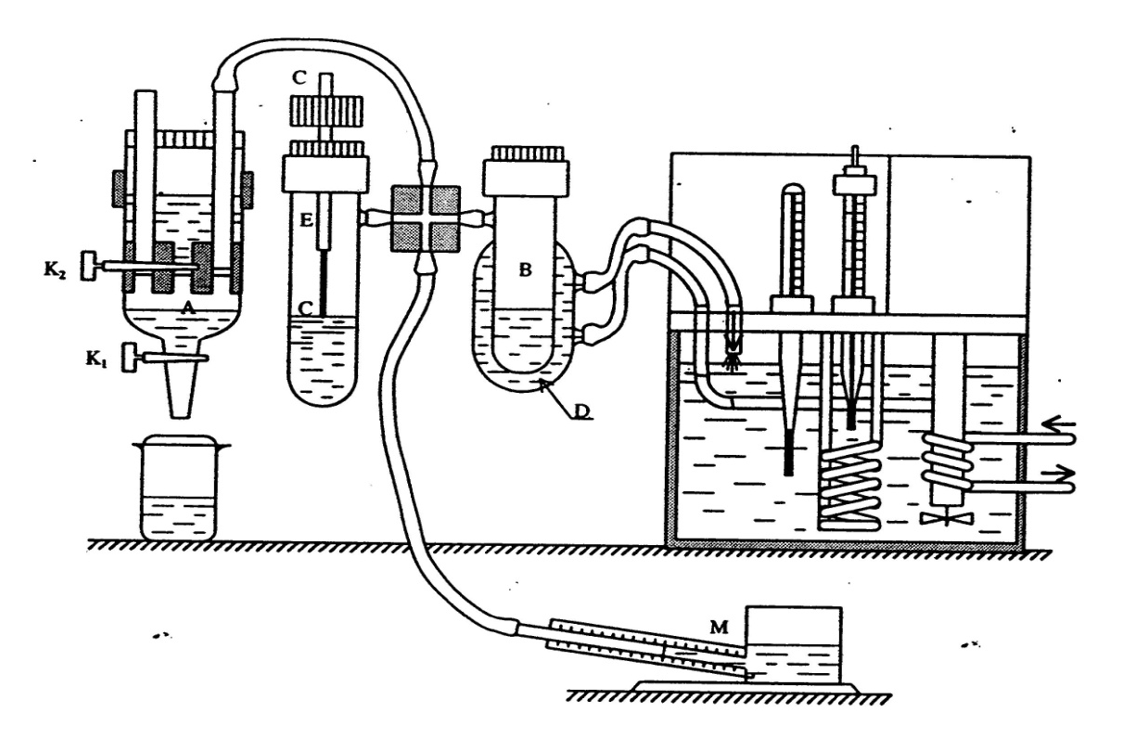
\includegraphics[width = 0.7\textwidth]{setup.PNG}
    \caption{Схема экспериментальной установки}
    \label{fig:setup}
\end{figure}

В работе использован прибор Ребиндера, изображённый на рис. \ref{fig:setup}. Исследуемая жидкость (дистиллированная вода) наливается в колбу В, тестовая жидкость (этиловый спирт) - в сосуд Е (см. рис. \ref{fig:setup}). При измерениях колбы герметично закрываются пробками. Через одну из двух пробок проходит полая металлическая игла С. Этой пробкой закрывается сосуд, в котором  проводятся измерения. Верхний конец иглы открыт в атмосферу, а нижний погружен в жидкость. Другой сосуд герметично закрывается второй пробкой. При создании достаточного  разряжения воздуха в колбе с иглой пузырьки воздуха начинают пробулькивать через жидкость. Поверхностное натяжение можно определить по величине разряжения $\Delta P$, необходимого для прохождения пузырьков.
Разряжение в системе создается с помощью аспиратора А. Кран К2 разделяет две полости аспиратора. Верхняя полость при закрытом кране К2 заполняется водой. Затем кран К2 открывают и заполняют водой нижнюю полость аспиратора. Разряжение воздуха создается в нижней полости при открывании крана К1, когда вода вытекает из неё по каплям. В колбах В и С, соединённых трубками с нижней полостью аспиратора, создается такое же пониженное давление. Разность давлений в полостях с разряженным воздухом и атмосферой измеряется спиртовым микроманометром, расположенным под углом к поверхности. Полное давление $P$, измеренное микроманометром, равно

\begin{equation}
    P = \rho gh + \Delta P,
    \label{rhogh}
\end{equation}

где $\rho$ - плотность жидкости, $h$ - глубина погружения иглы. Для стабилизации температуры исследуемой жидкости через рубашку D колбы В непрерывно прогоняется вода из термостата.

\section{Оборудование и экспериментальные погрешности}

\textbf{В работе использовались:} прибор  Ребиндера  с термостатом и микроманометром; исследуемые жидкости - дистиллированная вода и спирт; микроскоп, линейка, термометр.

\textbf{Инструментальные погрешности:}

\begin{itemize}
    \item Линейка: $\Delta_l = 0,5$ мм;
    \item Микроскоп: $\Delta_d = 0,025$ мм;
    \item Микроманометр: $\Delta_h = 0,5$ мм;
    \item Термометр: $\Delta_T = 0,5$ К.
\end{itemize}

\section{Результаты измерений и обработка экспериментальных данных}

\subsection{Исследование жидкости с известным коэффициентом поверхностного натяжения}

Перед началом измерений с дистиллированной водой был проведён предварительный опыт со спиртом, коэффициент поверхностного натяжения которого известен, для проверки использованных в работе закономерностей. Пузырьки начали пробулькивать через спирт при максимальном давлении, соответствующем высоте столба спирта $h = 42$ мм. Разброс полученных значений настолько незначителен, что показания микроманометра не отличались в пределах его систематической погрешности. Давление определяется из показаний микроманометра в делениях $h$ и показателя наклона $k = 0,2$ как

\begin{equation}
    \Delta P = 9,81kh = 82,4 \text{ Па}.
    \label{micromano}
\end{equation}

Погрешность измерения давления термеометром равна $\Delta_P = 9,81k\Delta_h = 1,0$ Па.

Табличное значение коэффициента поверхностного натяжения спирта при комнатной температуре $\sigma_\text{сп} = 22,03 \cdot 10^{-3}$ Н/м. По формуле Лапласа \eqref{Laplass}
 
\begin{equation}
    d = \frac{4\sigma}{\Delta P} = 1,07 \text{ мм}.
\end{equation}

Измеренное микроскопом значение диаметра иглы составило $d = 1,15$ мм. Значения различаются менее чем на 10\%, что говорит о применимости формулы Лапласа в данном опыте.

\subsection{Измерение коэффициента поверхностного натяжения воды}

Далее были проведены опыты по измерению коэффициента поверхностного натяжения воды и его зависимости от температуры. При комнатной температуре $T = 296$ К было измерено гидростатическое давление на глубине $\Delta h = 15,5$ мм как разница давлений при полном погружении иглы ($h_2 = 201$) и при касании концом иглы поверхности воды ($h_1 = 134$):

\begin{equation}
    \rho gh = \Delta P_2 - \Delta P_1 = 9,81k(h_2 - h_1) = 131,5 \text{ Па}.
\end{equation}

Значение, измеренное непосредственно по формуле: $\rho gh = 152,1$ Па. Однако можно утверждать, что значение, измеренное микроманометром, более точно, так как точно оценить глубину погружения иглы и плотность воды использованными приборами затруднительно.

Далее в интервале от 20 до 60 $^\text{o}$C было измерено 7 значений разницы давлений в воде при разных температурах. По формулам \eqref{Laplass}, \eqref{rhogh} и \eqref{micromano} найдены соответствующие значения коэффициента поверхностного натяжения. Результаты измерений представлены в таблице \ref{tab:tensions}

\begin{table}[]
    \centering
    \begin{tabular}{|c|c|c|c|c|}\hline
        $T$, К & $h$, мм & $P$, Па & $\Delta P$, Па & $\sigma$, $10^{-3}$ Н/м \\ \hline
        296 & 201 & 394.4 & 262,9 & 75,57 \\ \hline
        301 & 200 & 392,4 & 260,9 & 75,01 \\ \hline
        306 & 198 & 388,5 & 257,0 & 73,88 \\ \hline
        311 & 196 & 384,6 & 253,1 & 72,75 \\ \hline
        316 & 194 & 380,6 & 249,1 & 71,62 \\ \hline
        321 & 192 & 376,7 & 245,2 & 70,50 \\ \hline
        326 & 190 & 372,8 & 241,3 & 69,37 \\ \hline
        331 & 188 & 368,9 & 237,4 & 68,24 \\ \hline
        \end{tabular}
    \caption{Температурная зависимость значения коэффициента поверхностного натяжения}
    \label{tab:tensions}
\end{table}

\begin{figure}
\centering
\resizebox {0.55\textwidth} {!} {
\begin{tikzpicture}
\begin{axis}[ xlabel = {$T$, К}, ylabel = {$\sigma$, $10^{-3}$ Н/м}, xmin = 295, xmax = 332, ymin = 68, ymax = 76, legend style={legend style={at={(axis cs:332, 76)},anchor=north east}}]
\addplot[color=black, mark=x, only marks] coordinates{
(296, 75.57)
(301, 75.01)
(306, 73.88)
(311, 72.75)
(316, 71.62)
(321, 70.5)
(326, 69.37)
(331, 68.24)};
\addplot[color=blue] coordinates{(295, 76.18)(332, 68.19)};

\end{axis}
\end{tikzpicture}
}
\caption{Зависимость коэффициента поверхностного натяжения воды от температуры}
\label{graph1}
\end{figure}

На рис. \ref{graph1} изображена зависимость $\sigma(T)$. С помощью метода наименьших квадратов можно построить аппроксимирующую прямую и оценить величину $d\sigma/dT$:

\begin{equation}
    k = \frac{d\sigma}{dT} = \frac{\langle \sigma T \rangle - \langle \sigma \rangle \langle T \rangle}{\langle T^2 \rangle - \langle T \rangle^2} = -0,216 \cdot 10^{-3} \text{ Н/м}\cdot\text{К}, 
\end{equation}

\begin{equation}
    b = \langle \sigma \rangle - k\langle T \rangle = 139,9 \text{ Н/м}.
\end{equation}

Погрешность определения коэффициента наклона прямой можно найти по формуле

\begin{equation}
    \sigma_k = \sqrt{\frac{1}{8}(\frac{\langle \sigma^2 \rangle - \langle \sigma \rangle^2}{\langle T^2 \rangle - \langle T \rangle^2} - k^2)} = 0,005 \text{ Н/м}\cdot\text{К}.
\end{equation}

Зная коэффициент поверхностного натяжения и его температурную зависимость, можно установить зависимости $q(T)$ и $U_F(T)$. Графики данных зависимостей представлены на рис. \ref{graph2} и \ref{graph3}.

\begin{figure}
\centering
\resizebox {0.55\textwidth} {!} {
\begin{tikzpicture}
\begin{axis}[ xlabel = {$T$, К}, ylabel = {$q$, $10^{-3}$ Дж/м$^2$}, xmin = 295, xmax = 332, ymin = 63, ymax = 72, legend style={legend style={at={(axis cs:332, 17)},anchor=north east}}]
\addplot[color=blue] coordinates{
(296, 64)
(301, 65.08)
(306, 66.17)
(311, 67.25)
(316, 68.33)
(321, 69.41)
(326, 70.49)
(331, 71.57)};

\end{axis}
\end{tikzpicture}
}
\caption{Зависимость теплоты образования единицы поверхности воды от температуры}
\label{graph2}
\end{figure}

\begin{figure}
\centering
\resizebox {0.55\textwidth} {!} {
\begin{tikzpicture}
\begin{axis}[ xlabel = {$T$, К}, ylabel = {$U_F/F$, $10^{-3}$ Дж/м$^2$}, xmin = 295, xmax = 332, ymin = 135, ymax = 145, legend style={legend style={at={(axis cs:332, 92.5)},anchor=north east}}]
\addplot[color=purple] coordinates{
(296, 139.58)
(301, 140.09)
(306, 140.05)
(311, 140)
(316, 139.95)
(321, 139.91)
(326, 139.86)
(331, 139.81)};
\end{axis}
\end{tikzpicture}
}
\caption{Зависимость полной энергии единицы поверхности воды от температуры}
\label{graph3}
\end{figure}

\section{Обсуждение результатов и выводы}

Табличные значения коэффициента поверхностного натяжения воды при комнатной температуре лежат в пределах 73-74$\cdot$10$^{-3}$ Н/м. Значения, полученные в ходе данной работы, отклоняются от табличных не более, чем на 2-5\%. Относительные систематические и случайные погрешности также не превышают нескольких процентов. Это говорит о том, что точность опыта достаточно высока и позволяет проверить экспериментально рассмотренные теоретические закономерности.

В ходе опыта было установлено, что зависимость поверхностного натяжения от температуры линейна. Это соответствует теоретическим сведениям: по правилу Этвёша коэффициент поверхностного натяжения воды определяется как

\begin{equation}
    \sigma \approx 0,073 (1 - 0,002 \cdot (T - 291)).
\end{equation}

Следовательно, использованная в данной работе экспериментальная установка позволяет с большой точностью измерить энергию поверхности воды в температурном диапазоне от 20 до 60 К.

\end{document}
